\section{Intro}

	\begin{frame}
		\begin{center}
			\LARGE{\tblue{Concetti introduttivi}}
		\end{center}
	\end{frame}

	\subsection{Concetti introduttivi}
	
		\begin{frame}
			\frametitle{Terminologia base}		
			I cinque ingredienti principali con cui lavoreremo sono:
			\begin{itemize}
				\item \tblue{Plaintext}: il messaggio originale da cifrare
				\item \tblue{Ciphertext}: il messaggio cifrato
				\item \tblue{Algoritmo di encryption}: l'algoritmo utilizzato per criptare il plaintext
				\item \tblue{Algoritmo di decryption}: l'algoritmo utilizzato per decriptare il ciphertext
				\item \tblue{Chiave segreta}: la chiave condivisa dalle parti fornita in input all'algoritmo di encryption
			\end{itemize}
		\end{frame}
		
		\begin{frame}
			\frametitle{Crittografia}		
			I sistemi crittografici sono generalmente classificati secondo tre dimensioni:
			\begin{itemize}
				\item Il tipo di operazioni effettuate sul plaintext (sostituzione o trasposizione)
				\item Il numero di chiavi usate
				\item Come il plaintext viene processato (blocchi o stream)
			\end{itemize}
		\end{frame}
	
		{\fontsize{10}{0}
		\begin{frame}
			\frametitle{Principi di Kerckhoffs}	
			Nel 1883 Auguste Kerckhoffs pubblicò ne \tblue{"La Cryptographie Militaire"} i principi progettuali per i cifrari militari	
			\begin{itemize}
				\item Il sistema deve essere praticamente, se non matematicamente, indecifrabile
				\item \tblue{Questo non deve essere segreto, deve essere in grado di cadere nelle mani del nemico senza inconvenienti}
				\item La sua chiave deve essere comunicabile senza l'aiuto di note scritte, e modificabile o modificabili a piacimento dei corrispondenti
				\item \textst{Deve essere applicabile alla corrispondenza telegrafica}
				\item \textst{Deve essere portatile} e il suo utilizzo non deve richiedere il concorso di più persone
				\item È necessario che la sua applicazione sia facile da usare e che non richieda la conoscenza e l'uso di una lunga serie di regole	
			\end{itemize}
		\end{frame}}
		
		\begin{frame}
			\frametitle{Tipi di attacchi di criptoanalisi possibili}		
			\begin{figure}
				\begin{center}
						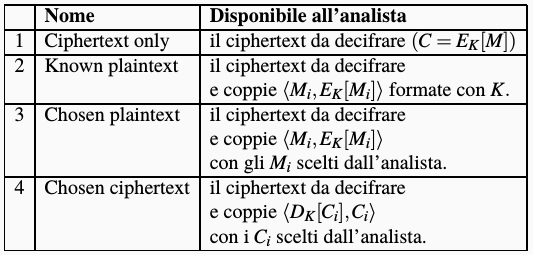
\includegraphics[scale = 0.45]{img/attacchi}
						\caption{Attacchi}
				\end{center}
			\end{figure}
		\end{frame}

